\subsection{CORS}
\label{subsec:S3_cors}

Cross-origin resource sharing (CORS) is a mechanism that allows restricted resources (e.g. fonts, JavaScript, etc.) on a web page to be requested from another domain outside the domain from which the resource originated.

A web page may freely embed images, stylesheets, scripts, iframes, videos and some plugin content (such as Adobe Flash) from any other domain. However embedded web fonts and AJAX (XMLHttpRequest) requests have traditionally been limited to accessing the same domain as the parent web page (as per the same-origin security policy).``Cross-domain'' AJAX requests are forbidden by default because of their ability to perform advanced requests (POST, PUT, DELETE and other types of HTTP requests, along with specifying custom HTTP headers) that introduce many cross-site scripting security issues.

CORS defines a way in which a browser and server can interact to safely determine whether or not to allow the cross-origin request. It allows for more freedom and functionality than purely same-origin requests, but is more secure than simply allowing all cross-origin requests. It is a recommended standard of the W3C.

The CORS standard describes new HTTP headers which provide browsers and servers a way to request remote URLs only when they have permission. Although some validation and authorization can be performed by the server, it is generally the browser's responsibility to support these headers and respect the restrictions they impose.

For AJAX and HTTP request methods that can modify data (usually HTTP methods other than GET, or for POST usage with certain MIME types), the specification mandates that browsers ``preflight'' the request, soliciting supported methods from the server with an HTTP OPTIONS request header, and then, upon ``approval'' from the server, sending the actual request with the actual HTTP request method. Servers can also notify clients whether ``credentials'' (including Cookies and HTTP Authentication data) should be sent with requests \cite{s3_cors}. 

\begin {figure}[h]
\graphicspath{{images/chapter_s3/}}
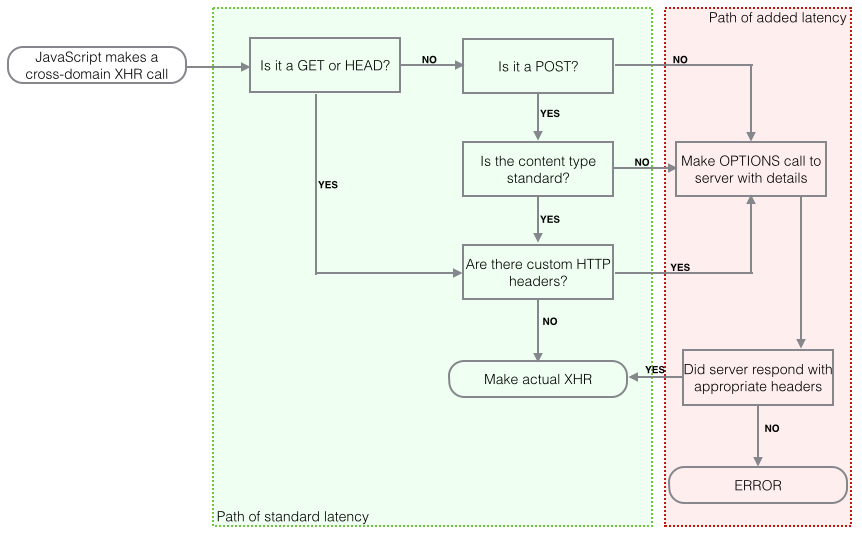
\includegraphics[width=\textwidth]{cors}
\caption{Flowchart showing Simple and Preflight XHR by Bluesmoon}
\end {figure}

